\chapter{FUNDAMENTAÇÃO TEÓRICA}

Este capítulo tem como objetivo apresentar os conceitos teóricos, padrões arquiteturais e tecnologias que embasam o desenvolvimento da plataforma qDATA. Ao longo das próximas seções, discutiremos as bases fundamentais necessárias para a compreensão das escolhas metodológicas detalhadas posteriormente, contextualizando-as no cenário de engenharia de software voltada a sistemas de alta disponibilidade e baixa latência.

Dada a natureza do problema do LTI, que exige a ingestão contínua de grandes volumes de dados financeiros (barras OHLC) e seu consumo em atividades internas do LTI, a infraestrutura projetada baseia-se fortemente em práticas modernas da indústria. Discorreremos sobre como conceitos consolidados, como microsserviços, conteinerização e comunicação híbrida via protocolos eficientes, sustentam os requisitos operacionais sem comprometer a estabilidade do serviço.

\section{O Ecossistema LTI FinHub}

O FinHub é um ecossistema abrangente desenvolvido no âmbito do Laboratório de Tecnologias Inovadoras (LTI). Trata-se de um sistema amplo que orquestra múltiplos serviços e componentes para viabilizar a pesquisa quantitativa avançada. A Figura \ref{fig:ecossistema_finhub} ilustra a arquitetura conceitual e a interação entre os diversos elementos que compõem este ambiente.

Neste trabalho, adotamos como ponto de partida inicial o componente qDATA, dedicando a ele um enfoque predominantemente técnico. Contudo, conservamos a perspectiva sistêmica de que o qDATA, embora seja um componente individual, desempenha um papel central e, portanto, precisa se relacionar adequadamente com os demais serviços do ecossistema. O sucesso de sua implementação depende da interoperabilidade harmoniosa com módulos como o \textit{feeder}, os painéis de visualização (\textit{dashboards}) e os futuros serviços de simulação.

Ademais, ressalta-se que o presente estudo consolida as bases infraestruturais. Um trabalho futuro (TCC2) dará ênfase a aspectos mais amplos, como governança de TI, aprofundamento na arquitetura de microsserviços e práticas de \textit{Product Ownership}, garantindo que a evolução do ecossistema FinHub ocorra de forma gerenciada, escalável e alinhada às necessidades estratégicas dos pesquisadores envolvidos.

\begin{figure}[htb]
    \centering
    \caption{Ecossistema LTI FinHub}
    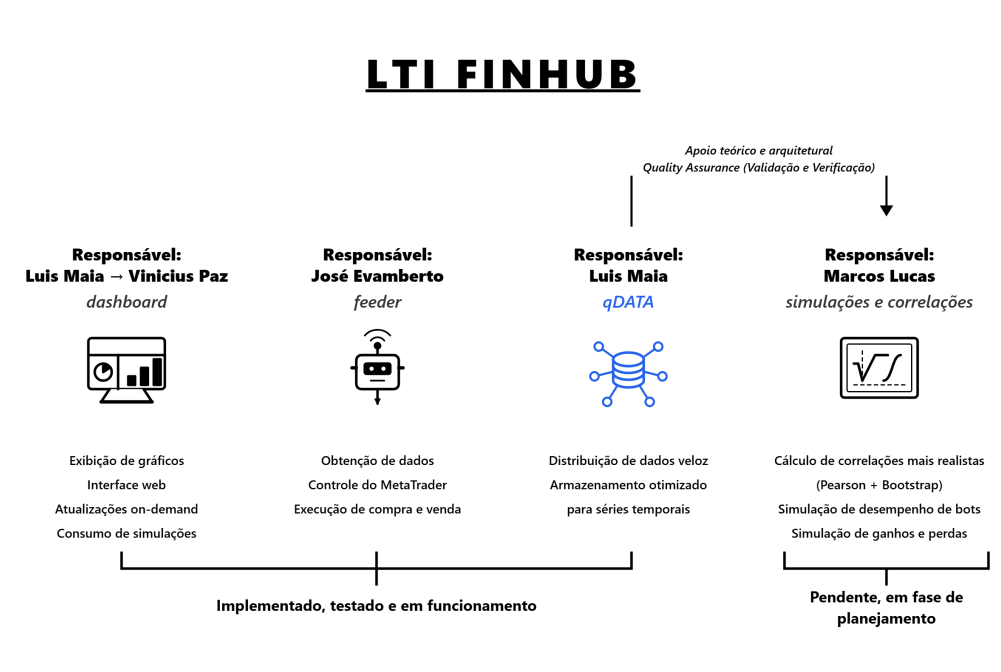
\includegraphics[width=\textwidth]{assets/figura_5_ecossistema_finhub.png}
    \label{fig:ecossistema_finhub}
\end{figure}

\section{Arquitetura de Microsserviços}

A arquitetura de microsserviços consiste em uma abordagem na qual uma única aplicação é composta por um conjunto de pequenos serviços, cada um executando seu próprio processo e comunicando-se por meio de mecanismos leves, geralmente \textit{Application Programming Interfaces} (APIs) sobre o protocolo \textit{Hypertext Transfer Protocol} (HTTP). Conforme postulado por \citeonline{newman2015building}, essa arquitetura enfatiza serviços independentemente implantáveis, construídos em torno de capacidades de negócios e com implantação automatizada.

\begin{comment}
Ao contrário de abordagens monolíticas — onde todos os componentes lógicos (interface, regras de negócio e acesso a dados) são empacotados juntos —, os microsserviços promovem um acoplamento fraco e alta coesão. Essa granularidade permite que equipes operem de forma descentralizada, atualizando um componente sem o risco de impactar a disponibilidade geral do sistema. Na engenharia de software para plataformas financeiras, a resiliência gerada pelo isolamento de falhas é de extrema importância.
\end{comment}

Ao contrário de abordagens monolíticas – onde todos os componentes lógicos (interface, regras de negócio e acesso a dados) são desenvolvidos dentro de um mesmo repositório – os microsserviços promovem um acoplamento mais fraco, e melhora a coesão. Evidentemente, essa melhoria não é absoluta, pois o desmembramento de um software grande em unidades menores pode impactar contratos, dependências, segurança ou a integração com outros serviços. Ainda assim, as vantagens citadas ultrapassa a mera organização arquitetural do código. 

Nesse sentido, conforme visto nos trabalhos dentro do laboratório, tal abordagem permitiu mais flexibilidade para a equipe, e membros da equipe podem se voluntariar a serem responsáveis por um componente específico. Uma prática interessantíssima nesse cenário é a atribuição a um membro de responsabilidade "end-to-end" por algum(s) serviço(s). Em outras palavras, é possível estruturar a organização do laboratório de modo que certos colaboradores sejam totalmente responsáveis por um serviço. Tal trabalho é, ainda, viabilizado pelo tamanho do serviço, que devido à modularização não representa um software inteiro, mas apenas um parte do todo.

No contexto deste trabalho, a arquitetura de microsserviços justifica a divisão estrutural entre o componente de coleta de dados (\textit{feeder}) e a plataforma centralizadora (qDATA). Ou seja, foi projetado para que as responsabilidades de (1) aquisição das séries temporais e de (2) armazenamento e distribuição sejam escaladas, monitoradas e mantidas de maneira totalmente autônoma.

Nesse contexto, destaca-se que uma versão inicial – e precária – do \textit{feeder} foi prototipada e usada em experimentos no projeto, mas a versão final e de qualidade só foi desenvolvida posteriormente, pelo discente José Evamberto Lima Oliveira, conforme descrito em seu trabalho \textit{Manutenção e Evolução do Sistema MT5-Websocket-Bridge no projeto de extensão LTI – Análise de séries financeiras} \cite{oliveira2026}.

\section{Coleta de Dados com Tickers Especializados}

A especialização em coleta de dados, por parte do discente José Oliveira, cujo trabalho se comunica diretamente com o meu, abriu caminho para três possibilidades de trabalho. Em primeiro lugar, possibilitou a divisão da carga de trabalho, permitindo que o trabalho do sistema de dados fosse dividido em duas partes menores, evitando a sobrecarga laboral.

Em segundo lugar, tornou possível a coleta especializada de tickers. Nesse sentido, cita-se o fato de que há dois tipos de tickers na biblioteca Python do Metatrader5. São eles: (1) \texttt{mt5.COPY\_TICKS\_TRADE}, que filtra a base de dados do MT5 e só te entrega os momentos em que um comprador e um vendedor fecharam negócio.

Em segundo lugar, temos o (2) \texttt{mt5.COPY\_TICKS\_INFO}, que traz apenas as atualizações do Book de Ofertas (Livro de Preços). Ou seja, alguém colocou, moveu ou cancelou uma ordem limite de compra (Bid) ou venda (Ask), mas nenhum negócio foi fechado. Ele é fortemente recomendado para trabalhos estatísticos, simulações, uso em estratégias de \textit{trading}, etc.

Por fim, temos o tipo de ticker (3) \texttt{mt5.COPY\_TICKS\_ALL} que traz absolutamente tudo. Cada vez que o Bid mudou, o Ask mudou, ou um negócio aconteceu, uma nova linha é gerada. Deve-se notar que o volume de dados gerado por essa flag é gigantesco, especialmente em ativos líquidos como mini-índice (WIN), um tipo ideal para trabalhos e técnicas estatísticas que dependem muito de volume.

Nesse contexto, no que tange aos \textit{stakeholders} do projeto, temos a possibilidade de ofertar à equipe e à coordenadora do projeto três tipos diferentes de dados para um mesmo ativo, que devem ser escolhidos conforme a necessidade de cada demanda. Concluindo, o trabalho realizado em cada um desses componentes se torna mais especializado, produzindo componentes de mais qualidade no produto final.

\section{Contêineres e Docker}

A conteinerização revolucionou a implantação de software ao oferecer uma virtualização em nível de sistema operacional (processo). O Docker despontou como a principal ferramenta para essa prática, permitindo que desenvolvedores empacotem uma aplicação com todas as suas dependências, bibliotecas e arquivos de configuração necessários em um único artefato portável \cite{merkel2014docker}.

Um dos maiores ganhos operacionais da utilização de contêineres é o princípio conhecido como "\textit{build once, run anywhere}" (construa uma vez, execute em qualquer lugar). Na prática, se o contêiner funciona no ambiente de desenvolvimento, seu comportamento será idêntico nos ambientes de teste, homologação e produção, erradicando a clássica síndrome do "na minha máquina funciona". Essa previsibilidade minimiza substancialmente o esforço logístico em implantações complexas.

No desenvolvimento do projeto, o Docker permite empacotar o código do banco de dados e o código do ASGI (FastAPI) sem expor a máquina hospedeira a configurações conflitantes, além de permitir rápida manutenção do banco de dados e \textit{deploys} mais seguros.

\subsection{Compatibilidade de Binários em Ambientes Linux (Wine)}

Ainda dentro do domínio da infraestrutura de contêineres, surge frequentemente a necessidade de compatibilizar binários compilados exclusivamente para a plataforma Windows em ambientes operacionais baseados em Linux. O MT5, terminal frequentemente mandatório para conexão com corretoras brasileiras (como XP, Rico e Clear), possui versões nativas unicamente para o ecossistema da Microsoft.

Para contornar tal barreira no Linux, convenciona-se utilizar a camada de compatibilidade Wine (\textit{Wine Is Not an Emulator}). Trata-se de um software que traduz as chamadas de sistema (API) do Windows para equivalentes no padrão \textit{Portable Operating System Interface} (POSIX) do Linux em tempo real, evitando os atrasos de desempenho característicos de emuladores convencionais ou máquinas virtuais pesadas \cite{winehq2026}.

\section{Separação de Preocupações (Separation of Concerns)}

O princípio da Separação de Preocupações, originário dos primórdios da Ciência da Computação, determina que um sistema deve ser estruturado em seções distintas, onde cada seção lida com um conjunto específico e delineado de informações e tarefas. Um módulo deve ter uma, e apenas uma, razão primária para sofrer modificações.

Em sistemas distribuídos modernos, aplicar esse princípio significa evitar componentes "Deus", isto é, objetos ou serviços que sabem e fazem demais, um fenômeno discutido nas aulas de Programação Orientada a Objetos. Ao delegar as preocupações de obtenção de dados de mercado para um sistema dedicado, libera-se a ferramenta consumidora da tarefa de gerenciar autenticações complexas de API ou manter a resiliência de \textit{sockets} contínuos, focando unicamente na análise dos dados em si. Mais do que isso: essa arquitetura permitiu delegar a responsabilidade do "Departamento de Aquisição de Dados" (figura de linguagem) a um gerente dedicado especificamente a isso.

No domínio do Laboratório de Tecnologias Inovadoras, a adoção incisiva deste conceito molda a justificativa central do trabalho. O qDATA concentra-se puramente em agir como infraestrutura de dados compartilhada (\textit{Market Data}). A lógica de análise quantitativa, o treinamento de modelos estocásticos e a execução de ordens nas corretoras permanecem estritamente sob responsabilidade do cliente (\textit{researcher}). Essa fronteira rígida protege o núcleo do sistema de \textit{bugs} advindos de modelos preditivos em fase de experimentação.

\section{Protocolos de Comunicação: REST/HTTP e gRPC}

A intercomunicação eficaz é o coração de qualquer arquitetura de serviços distribuídos. O REST (\textit{Representational State Transfer}), introduzido por \citeonline{fielding2000}, tornou-se o padrão \textit{de facto} na web, caracterizado por sua operação \textit{stateless} sobre HTTP e pela ampla adoção global por sua clareza de uso. Contudo, em virtude de tradicionalmente carregar respostas verbosas em texto \textit{JavaScript Object Notation} (JSON) e depender de conexões repetidas no HTTP/1.1, a comunicação REST costuma esbarrar em gargalos quando exigida baixa latência e alta vazão (milhões de eventos por minuto).

Em contrapartida, o gRPC (\textit{gRPC Remote Procedure Call}) é um \textit{framework} moderno, focado em alta performance, que utiliza o protocolo HTTP/2 subjacente e o formato de serialização binária Protocol Buffers (Protobuf). Ele viabiliza não apenas chamadas incisivamente menores e mais rápidas no envio por rede, como também introduz o conceito valioso de conexões multiplexadas e o \textit{streaming} bidirecional de mensagens contínuas, mantendo o canal perenemente aberto \cite{google2016grpc}. Em outras palavras, conseguimos enviar múltiplas requisições por um mesmo canal \textit{Transmission Control Protocol} (TCP) em paralelo de um ponto de vista lógico, aumentando a performance da rede, e delegando a responsabilidade de controle de fluxo para o protocolo HTTP/2, que é otimizado para esse tipo de comunicação.

Adotamos, portanto, uma arquitetura de rede híbrida alinhada com as melhores práticas da indústria financeira. A ingestão de barras (\textit{feeder} enviando ao núcleo) ocorre via \textit{endpoints} REST baseados no HTTP clássico, permitindo fácil inspeção, monitoramento com \textit{webhooks} e integração simplificada. Simultaneamente, a distribuição dos dados temporais para o painel (\textit{dashboard}) dos pesquisadores é trafegada via canais gRPC otimizados, superando obstáculos inerentes ao JSON e minimizando fortemente a latência nas consultas volumosas de cotações históricas. Esclarecemos que a melhoria feita ao usar Protocol Buffers (Protobuf) em vez de JSON consiste no fato que esse tipo de serialização é mais compacta, além de ser mais rápida para serializar e desserializar em comparação ao formato de texto (JSON, \textit{Extensible Markup Language} (XML), etc). Nesse sentido, definimos serialização e desserialização como o processo de converter um objeto entre um formato utilizável pela memória do computador e um formato utilizável para transmissão ou armazenamento.

\section{Bancos de Dados para Séries Temporais: TimescaleDB}

Dados financeiros em formato OHLC (\textit{Open, High, Low, Close}) apresentam o caráter uníssono e linear de séries temporais (\textit{time-series}). Os bancos de dados relacionais tradicionais, embora robustos nas consultas transacionais simples e cruzamentos complexos (JOINs), frequentemente demonstram acentuada degradação em desempenho e crescimento descontrolado no espaço de armazenamento físico à medida em que as tabelas acumulam centenas de milhões de pontos sequenciais de observação no tempo.

A extensão de Postgres denominada "TimescaleDB" se projeta essencialmente como uma ferramenta voltada à adequação do Sistema de Gerenciamento de Banco de Dados (SGBD) padrão PostgreSQL aos exigentes critérios de \textit{Time-Series Data}. Seu principal diferencial repousa nas chamadas \textit{hypertables}: na superfície atuam identicamente como tabelas relacionais clássicas, no entanto operam no interior criando e gerenciando o particionamento dinâmico automático em blocos temporais isolados \cite{timescale2017}.

Desta forma, os pesquisadores do LTI podem submeter requisições envolvendo densas estatísticas com cálculos de médias e consolidação dos volumes intradiários em escalas cronológicas maiores (através das funções nativas como \texttt{time\_bucket}). O mecanismo subjacente somente inspeciona as frações de dados contidas nos intervalos requeridos (sem necessidade de percorrer todos os registros contidos em base de dados), e utiliza ainda algoritmos de compressão columnar sofisticados que propiciam economia substancial do espaço em disco sem sacrifício da presteza das consultas.

\section{FastAPI e Programação Assíncrona (ASGI)}

Com o advento e adoção crescente de ambientes concorrentes de \textit{Input/Output} (I/O), o padrão Python \textit{Asynchronous Server Gateway Interface} (ASGI) (\textit{Asynchronous Server Gateway Interface}) ascendeu para solucionar o bloqueio síncrono que assolava seus antecessores (como o Web Server Gateway Interface). O padrão ASGI gerencia requisições paralelamente de forma assíncrona, o que significa que a \textit{thread} do servidor pode atender a outras chamadas web sem travar a execução enquanto aguarda por respostas de tráfego de redes externas ou resoluções de consultas morosas no banco de dados.

O \textit{framework} FastAPI constrói-se exatamente sob essa base arquitetural assíncrona, ancorando suas credenciais de escalabilidade. Notabilizado pelo elevado e provado desempenho — equiparável a \textit{frameworks} baseados em Node.js e até mesmo linguagens compiladas como Go —, o FastAPI inclui documentação automatizada nativa (Swagger UI e ReDoc), e integra de maneira transparente a validação estrita de parâmetros das rotas por meio do robusto ecossistema de validação e tipagem "Pydantic" \cite{ramirez2018fastapi}.

Na engenharia do qDATA, essa capacidade de escalar perante tráfego denso foi determinante na seleção do FastAPI para hospedar a camada REST \textit{controller} do microsserviço central. O fluxo ininterrupto de dezenas (ou centenas) de \textit{feeders} simultâneos despejando as atualizações do índice a cada minuto causaria um enfileiramento nocivo numa estrutura web linear, ao passo que em regime assíncrono o banco de dados e a rede resolvem as requisições recebidas com sobreposição altamente otimizada. Cabe destacar que embora o serviço de distribuição de dados tenha sido feito com gRPC, a alimentação dos dados foi implementada via \textit{endpoints} REST/HTTP de recepção de dados. Essa escolha foi feita por questões de tempestividade do projeto, além do fato de que o gargalo desse ecossistema é a distribuição, e não a ingestão.

\section{Estratégia de Upsert e Idempotência}

Sistemas distribuídos convivem invariavelmente com o modelo de entrega na rede conhecido como "pelo menos uma vez" (\textit{at-least-once}), o que indica que repetições não intencionais de requisições ou atrasos são corriqueiros mediante instabilidades de conectividade. Para ingerir ininterruptamente um extenso número de barras de ativos e neutralizar os duplos envios na rede ou reconexões espontâneas do \textit{feeder}, não basta contar puramente com validações lógicas na camada da aplicação do servidor. É imperativa uma lógica sistêmica de banco de dados para prevenção à duplicação de anomalias temporais.

O mecanismo de \textit{Upsert} constitui o ato conjugado e atômico de inserir um registro se este for perfeitamente novo na persistência e, em oposição, efetuar estritamente uma atualização no registro já contido caso este fira metadados imutáveis pré-condicionados (as chaves concorrentes primárias). No dialeto moderno do banco de dados PostgreSQL, invoca-se essa característica via instrução \texttt{INSERT ON CONFLICT DO UPDATE}. Neste projeto, isso foi feito utilizando a função \texttt{merge} do \textit{Object-Relational Mapping} (ORM) (Object-Relational Mapping) do SQLAlchemy. Essa mescla transacional provê atualização sem carecer empenhar dispendiosos travamentos de linha (\textit{row locks}) longos no processo.

Para que as consultas gRPC entreguem aos painéis dos pesquisadores gráficos perfeitamente sincronizados, isentos de contaminações das séries e saltos matemáticos fictícios, os barramentos de injeção aplicam em profundidade este corolário. Na eventualidade de os \textit{feeders} retransmitirem parcelas horárias previamente já introduzidas, a abordagem \textit{Upsert} consolida a consistência atômica. É, portanto, garantida a premissa de \textit{Idempotência}: requisições idênticas com os mesmos parâmetros reproduzirão exatamente a mesma resultante estável a despeito das eventuais repetições impostas pelo emissor.

\section{Autenticação e Autorização com JWT e Supabase}

Garantir o livre mas vigiado intercâmbio de dados de mercado requer o uso de robustos arcabouços de gestão de identidade e acesso entre sistemas. O token JWT (\textit{JSON Web Token}) fornece a assinatura unificada baseada em um corpo de formato JSON codificado que detém asserções (\textit{claims}) prévias. Tais \textit{claims} validam a legitimidade sem impor onerosas revisões sistêmicas (pesquisas na tabela de sessão do banco) em cada requisição transacionada via rede, seguindo fidedignamente o padrão aberto da indústria formulado no \textit{Request for Comments} (RFC) 7519 do \textit{Internet Engineering Task Force} (IETF) \cite{rfc7519}. Em outras palavras, realizamos autenticação utilizando processamento lógico, em vez de consulta a um banco de dados, o que é mais eficiente e escalável. Notavelmente, a obtenção de um JWT válido, um processo que é feito apenas uma vez por sessão, envolve um banco de dados. Isto não é problemático, pois uma sessão pode durar horas ou dias, conforme o critério do engenheiro que desenhou as configurações do JWT. Haja vista que o domínio do presente trabalho se concentra em redes, sistemas distribuídos, e dados financeiros, utilizamos uma solução de nível mais alto e maior simplicidade para lidar com o manejo e autenticação dos usuários. Mais especificamente, utilizamos o Supabase para gerenciar quem tem permissão para receber um token JWT válido.

Dessa forma, esses \textit{tokens} são distribuídos por um \textit{Backend as a Service} (BaaS) (\textit{Backend as a Service}) \cite{supabase2020}. A implementação futura de Políticas de Segurança Orientadas a Linhas (\textit{Row Level Security} - RLS) do PostgreSQL aliado ao gerenciamento contínuo das credenciais — sem sobrecarregar nosso código próprio de engenharia com tratamento complexo de senhas — representa o estado da arte das soluções para gerência de perfis e controle de acesso seguro.

Com essa proteção validada e autossuficiente via JWT, as interações entre os variados pesquisadores e o grupo diretor principal do LTI ganham controles finamente ajustados de permissão e isolamento granular. Ao invés da tradicional adoção de um gargalo de API Gateway obsoleto centralizando a autorização primária de forma bloqueante, os próprios microsserviços atestam localmente de forma criptográfica (na verificação de chaves assimétricas públicas) a permissão adequada requerida para leitura do \textit{streaming} das cotações.

\section{Desenvolvimento Incremental e Integração Contínua}

Em contraponto às abordagens metodológicas clássicas e estritas de Cascata, metodologias contemporâneas ágeis pregam os aprimoramentos graduais focados em validação rápida ao invés do dispêndio excessivo na abstração estática e antecipada do projeto. A essência do Desenvolvimento Incremental consiste no adorno iterativo de pequenos recursos (ou subcomponentes funcionais da aplicação) dispostos contínua e ordenadamente sobre uma fundação com forte padronização contratual nas interfaces de comunicação do sistema. Admito que uma preocupação quanto à Engenharia de Software é a possibilidade de que o desenvolvimento incremental se reduza ao mero trabalho \textit{ad-hoc}.

No entanto, os avanços em ferramentas de linguagem natural têm avançado o desenvolvimento incremental a partir da criação de planos detalhados com mais facilidade, tanto antecipando problemas arquiteturais quando apontando ou criando possibilidades para evolução. Essa maleabilidade análise técnica do código e codificação aumentada (\textit{augmented coding}), evoluíram a prática de \textit{Continuous Integration} / Integração Contínua (CI). No mais, conforme a disponibilidade de tempo, uma lista de tarefas simples (\textit{task list}) pode ser utilizada para determinar (especificar) a utilização de algumas técnicas de engenharia, tal como requerer a construção de um Diagrama de Classes bem feito para representar a estrutura do código, um Diagrama de Atividades para especificar o processo de autenticação e consumo de dados, e um Diagrama de Sequência, que é mais crítico, para representar a interação entre os micro-serviços do ecossistema. Tem se tornado mais claro que este último diagrama seria crítico, pois no início do projeto tínhamos apenas o qDATA, o \textit{feeder} e o \textit{dashboard}, porém durante a criação deste TCC emergiu no LTI a necessidade de um micro-serviço de simulação de correlações \textit{bootstrapped}.

Esse novo cenário abre margem para a consolidação do uso de estratégias de orquestração de múltiplos repositórios (como submódulos e ferramentas de governança de código), um diferencial crucial no que tange à garantia de intercompatibilidade versional e à construção sustentável de ecossistemas de microsserviços. No Git, isso é feito com a função de submódulos, usando o comando \texttt{git submodule add} para adicionar um repositório dentro de outro. O submódulo é uma referência a um \textit{commit} específico do repositório externo, e o Git mantém o controle dessa referência. Assim, quando alguém clona o repositório principal, ele pode usar o comando \texttt{git submodule update --init --recursive} para baixar os submódulos e garantir que as versões corretas sejam usadas.

Dessa forma, a adoção de um \textit{pipeline} de CI robusto e automatizado, utilizando ferramentas como GitHub Actions, Jenkins ou GitLab CI/CD, é imperativa para o sucesso do projeto. O \textit{pipeline} deve incluir etapas de construção, testes automatizados (unitários, de integração e de regressão), análise estática de código e validação de segurança. Isso assegura que cada alteração no código seja rigorosamente verificada antes de ser integrada ao ramo principal, mantendo a estabilidade e a qualidade do sistema à medida que ele evolui. Como dito antes, tal fato não era tão evidente no estado inicial do ecossistema, pois existem apenas três aplicações: (1) qDATA, (2) MT5-Websocket-Bridge, e (3) o \textit{dashboard}. Todavia, à medida que o projeto cresce e mais componentes são adicionados – como o (4) Serviço de Simulações com Bootstrapping – a importância de um \textit{pipeline} de CI bem estruturado se torna ainda mais crítica para garantir a coesão e a integridade do sistema como um todo.
